\documentclass[parskip=full,11pt]{scrartcl}
\usepackage[utf8]{inputenc}

\title{\Huge Parkview\\
    \LARGE \normalfont Performance Dashboard for Continuous Benchmarking of HPC Libraries}
\author{Chingun Ariunbat, Jamil Bagga, Walter Alexander B\"ottcher,\\Darius Schefer, Maximilian Schik}

% section numbers in margins:
\renewcommand\sectionlinesformat[4]{\makebox[0pt][r]{#3}#4}

% header & footer
\usepackage{scrlayer-scrpage}
%\lofoot{\today} % Date in footer
\refoot{\today}  % no idea what this does
\pagestyle{scrheadings}

\usepackage[sfdefault,light]{roboto}
\usepackage[T1]{fontenc}
\usepackage[english]{babel}
\usepackage[yyyymmdd]{datetime} % must be after babel
\usepackage{float}
\renewcommand{\dateseparator}{-}
\usepackage[colorlinks=true, linkcolor=blue]{hyperref}
\usepackage{amsmath} % for $\text{}$
\usepackage[nameinlink]{cleveref}
\crefname{figure}{Abb}{Abb}
\usepackage[section]{placeins}
\usepackage{xcolor}
\usepackage[nonumberlist, toc]{glossaries}     % provides glossary commands, [toc] to appear in table of contents
\usepackage{graphicx}
\usepackage{dirtree}
\usepackage{listings}
\graphicspath{ {./images/} }
\hypersetup{
	pdftitle={Manual},
	bookmarks=true
}
\usepackage{manual}
\usepackage{csquotes} % provides \enquote{} command


\begin{document}

\maketitle
\begin{figure}[h]
	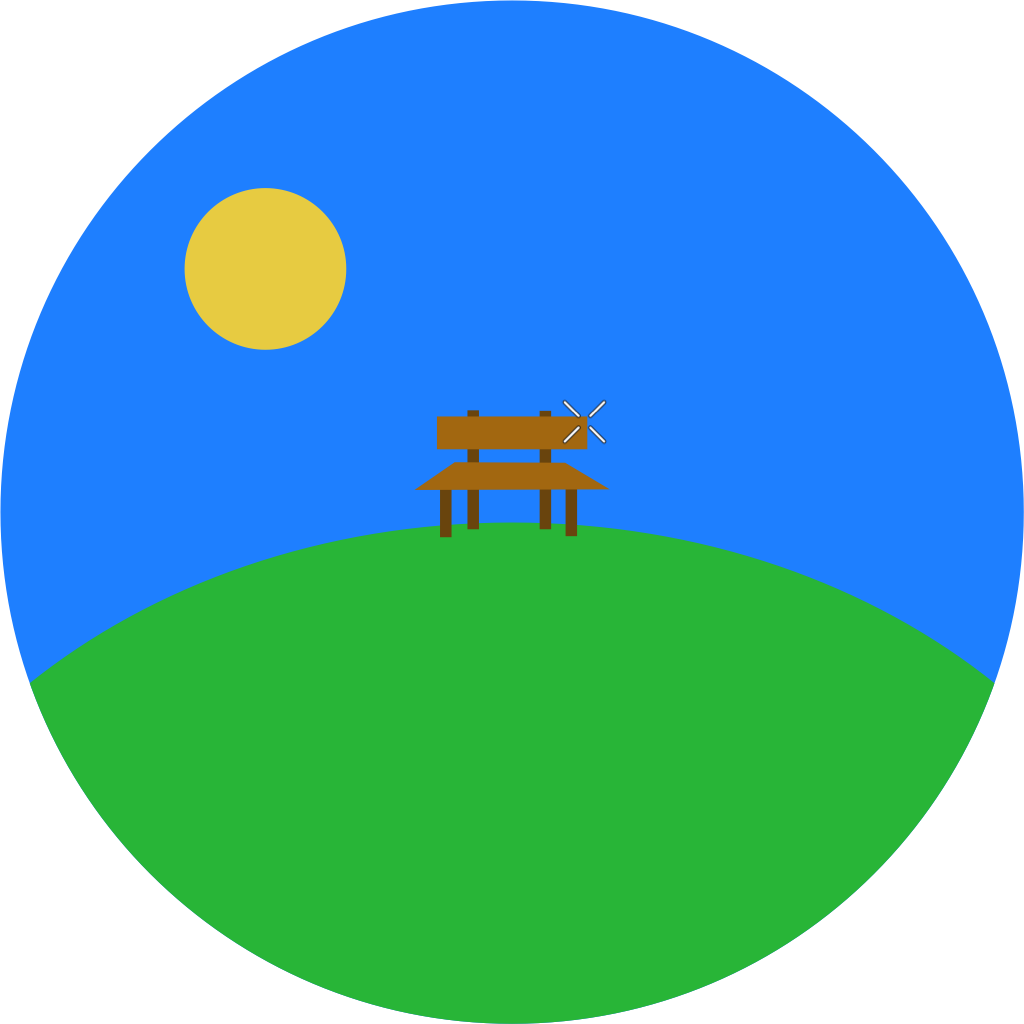
\includegraphics[width=11cm]{parkview.png}
	\centering
\end{figure}

\thispagestyle{empty}

\clearpage
\pagenumbering{arabic}

\tableofcontents
\clearpage

\section{Introduction}

Performance Dashboard for Continuous Benchmarking of HPC Libraries

PSE SS21

\section{System Overview}

The basic shape of the application stayed the same, with the backend handling data storage and processing, and the frontend requesting and visualizing data from the backend. \autoref{fig:system-model} gives a high level overview of all the important components.

\begin{figure}[h]
	\centering
	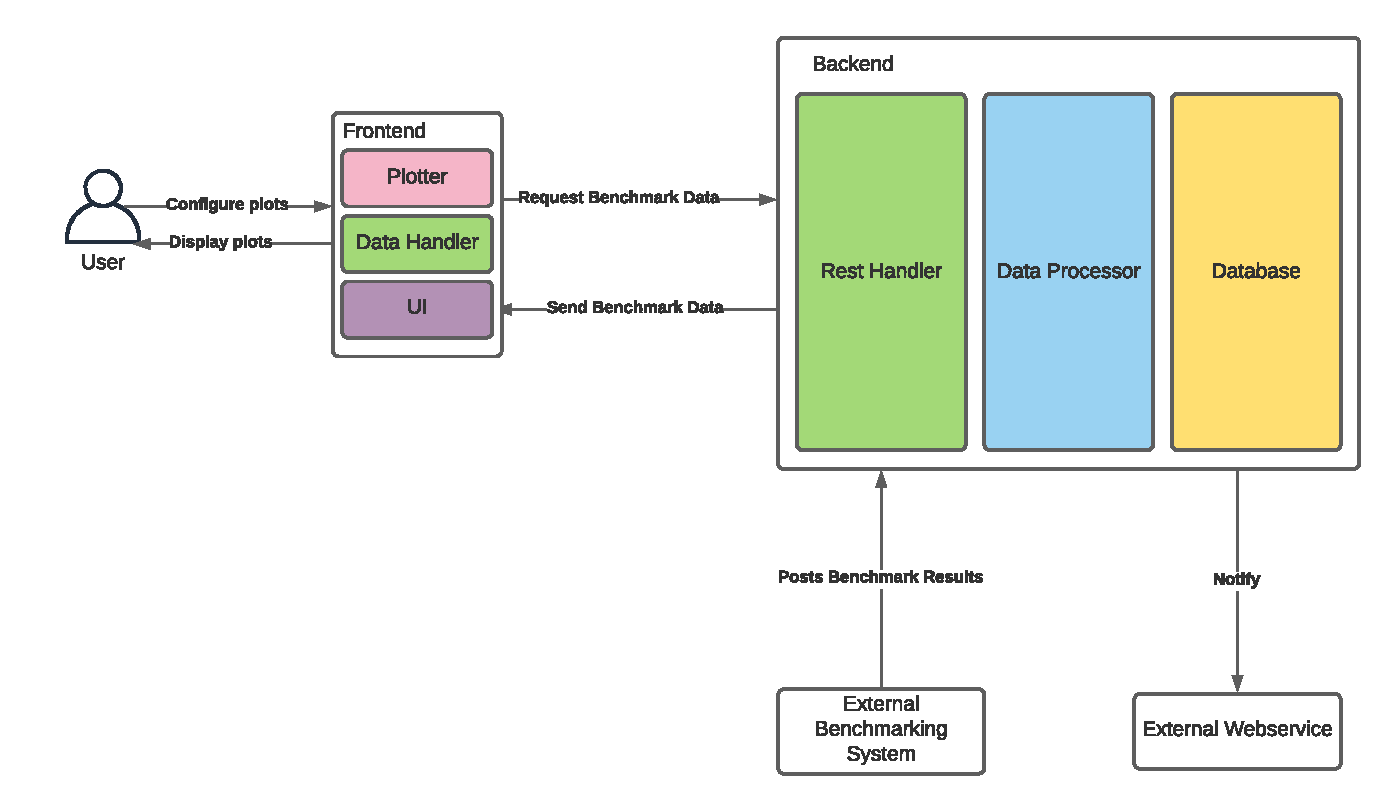
\includegraphics[width=\textwidth]{systemmodel.pdf}
	\caption{System Model}
  \label{fig:system-model}
\end{figure}

\subsection{Backend}
\begin{figure}[H]
	\centering
	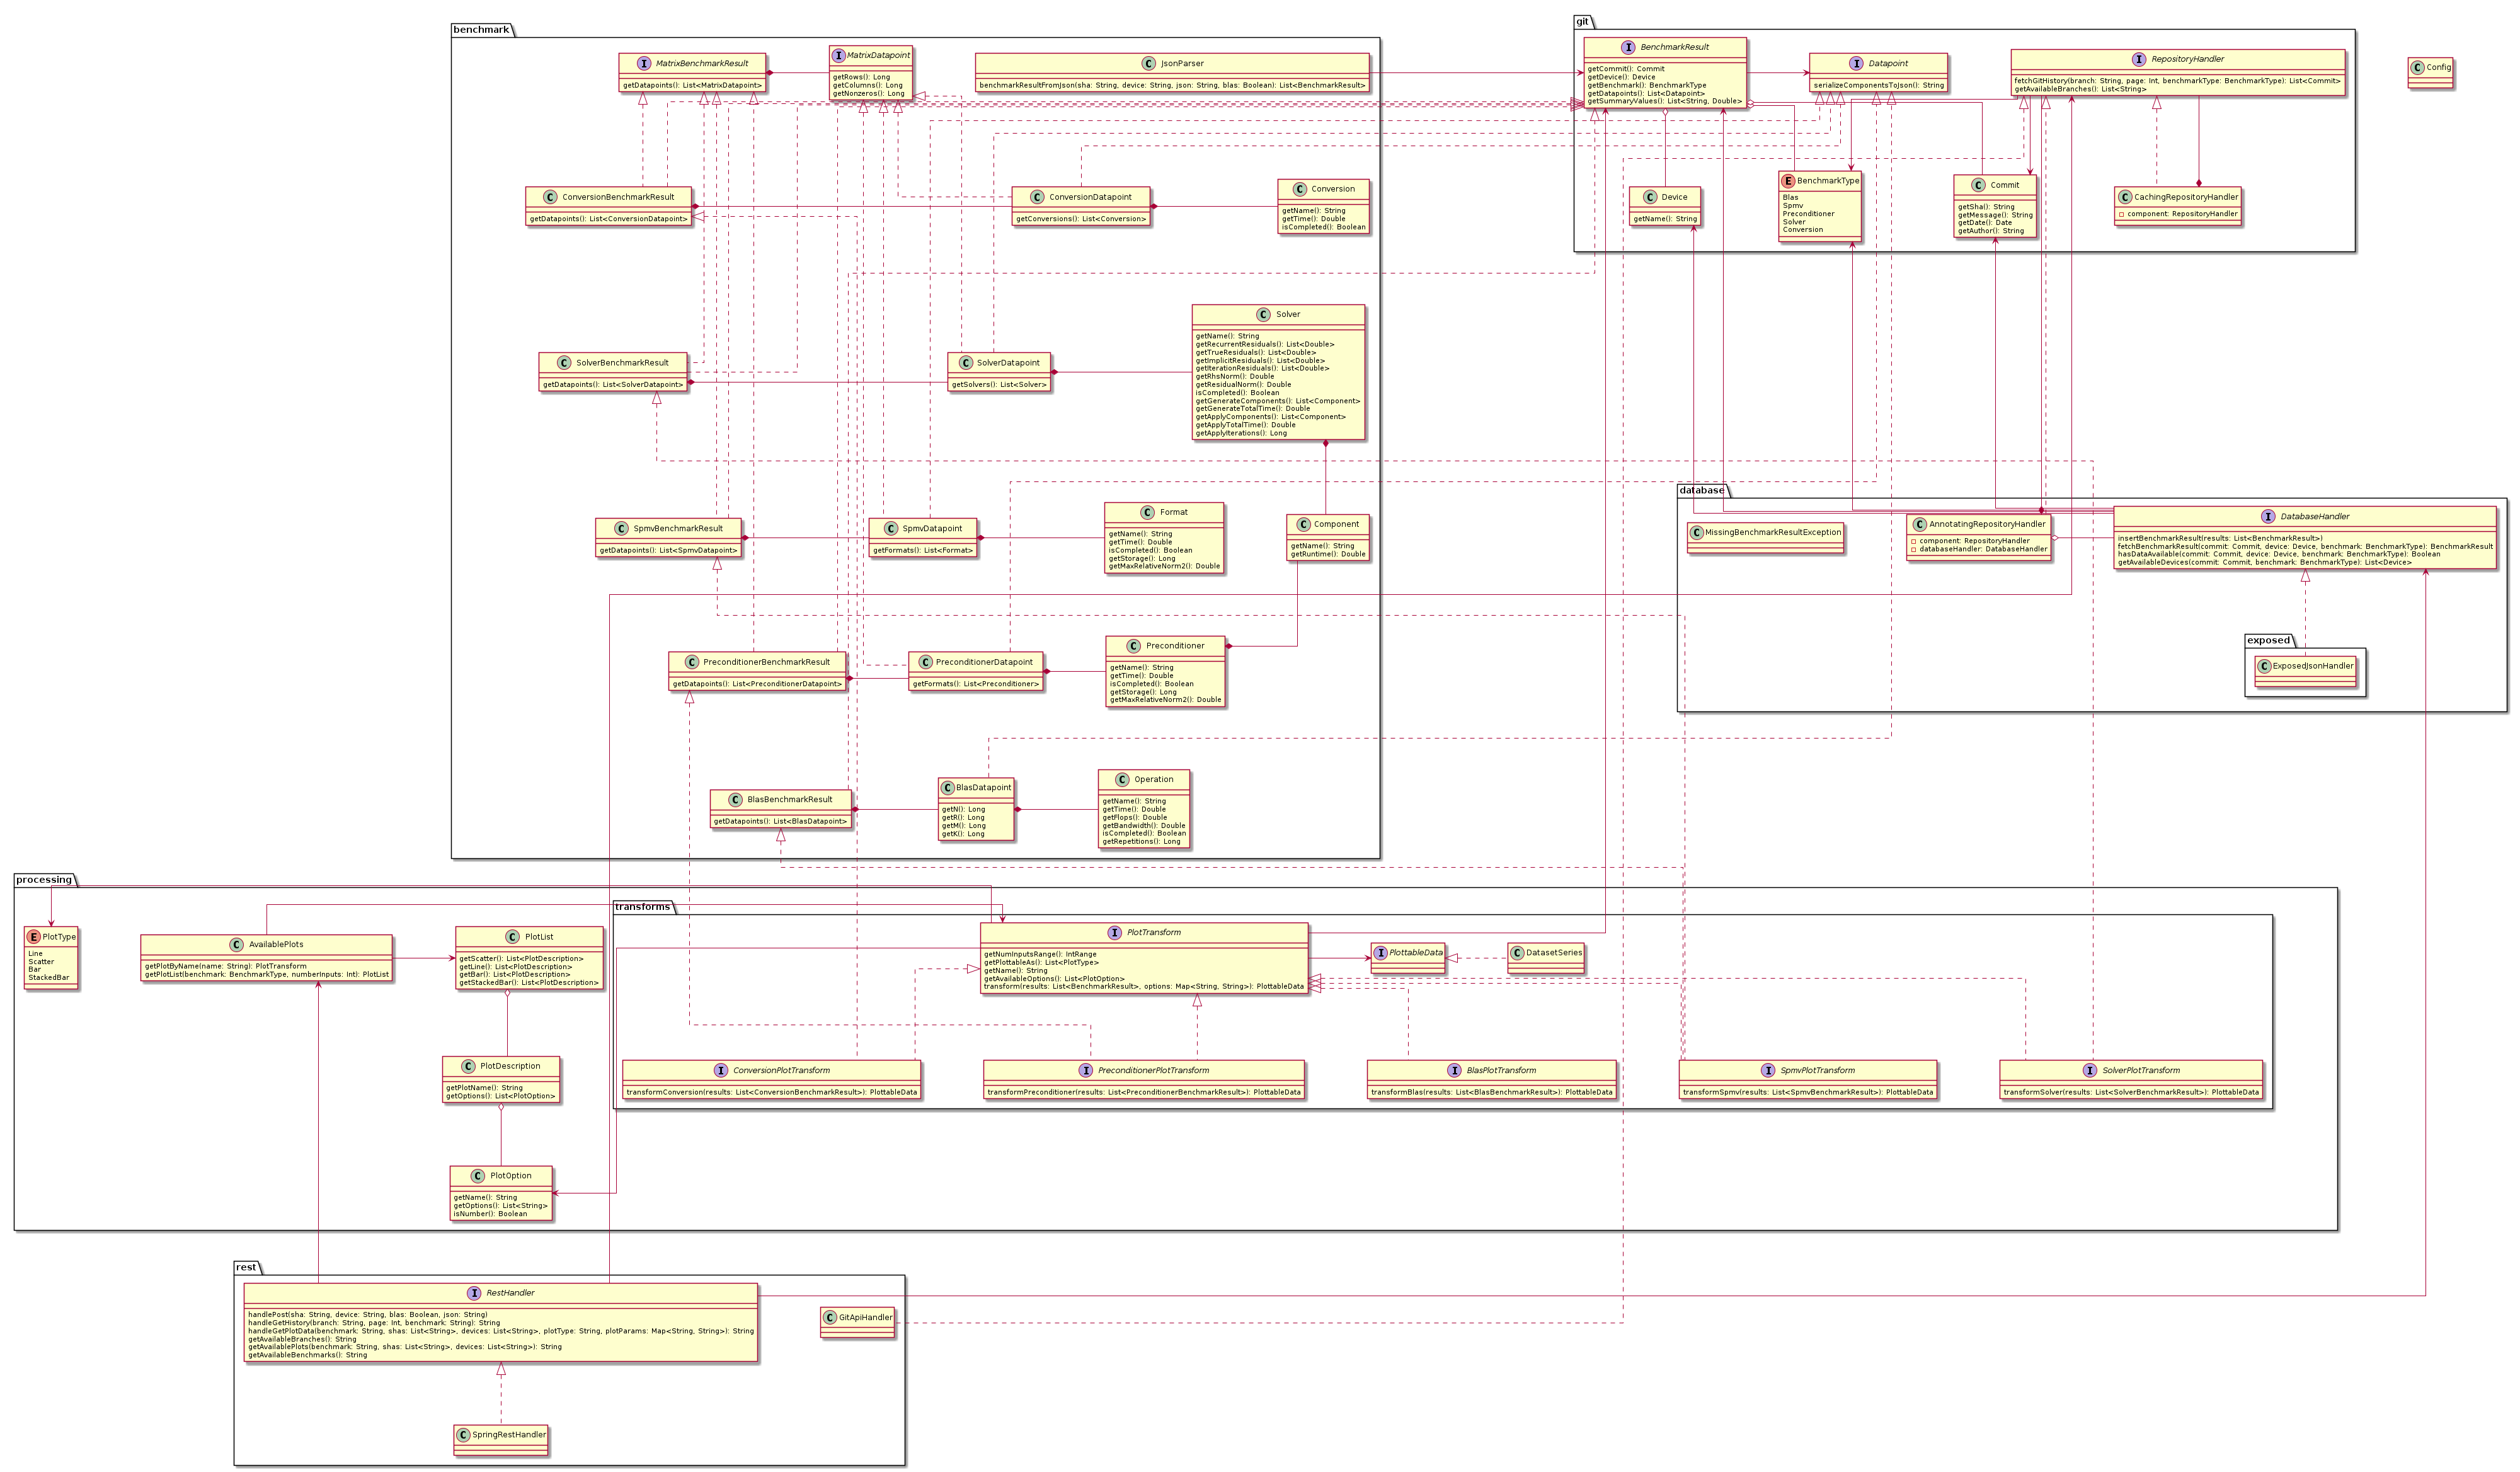
\includegraphics[width=\textwidth]{backend.png}
	\caption{UML class diagram for the backend}
  \label{fig:backend-class}
\end{figure}

The most important class/interface here is \texttt{PlotTransform}. It models transforms from benchmark results to plottable data. Every plot transformation implements this interface. Following is a more in depth description of the interface members:

\begin{itemize}
  \item \identifier{val numInputsRange:IntRange}{Range of allowed number of inputs. Since some plots can only take a single benchmark result and some can take multiple, this has to be defined. It should be mentioned that Kotlin offers some syntactic sugar for ranges, for example the range from one to ten can be represented by just \texttt{1..10}.}
  \item \identifier{val plottableAs:List<PlotType>}{Lists all plot types that can represent this transform. It uses the \texttt{PlotType} enum for that. This information is mainly for the frontend, since it has to know what plot to use.}
  \item \identifier{val name:String}{Name of transform, it has to be unique across all registered plot transforms}
  \item \identifier{fun getAvailableOptions(results:List<BenchmarkResult>):List<PlotOption>}{Returns a list of all available plot options, each containing a list of allowed values.}
  \item \identifier{fun transform(results:List<BenchmarkResult>):PlottableData}{Function that does the actual transforming. Usually you don't override this exact function because you implement one of the "subinterfaces" like \texttt{SpmvPlotTransform} which already overwrote that function and does some type and error checking. Instead you would override \texttt{fun transformSpmv(results:List<SpmvBenchmarkResult>):PlottableData} }
\end{itemize}

A quick example would be this snippet taken from \texttt{SpmvSingleScatterPlot}:

\begin{lstlisting}[style=JAVA]
class SpmvSingleScatterPlot : SpmvPlotTransform {
    override val numInputsRange = 1..1
    override val plottableAs = listOf(PlotType.Scatter)
    override val name = "spmvSingleScatterPlot"
    override fun getAvailableOptions(results: List<BenchmarkResult>): List<PlotOption> = listOf(
        PlotOption(
            name = "yAxis",
            options = listOf("bandwidth", "time"),
        ),
        PlotOption(
            name = "xAxis",
            options = listOf("nonzeros", "rows", "columns"),
        ),
    )

    override fun transformSpmv(
        benchmarkResults: List<SpmvBenchmarkResult>,
        options: Map<String, String>
    ): PlottableData {
      // transform code
    }
}
\end{lstlisting}

This is a transform for the SPMV benchmark, so it implements the \texttt{SpmvPlotTransform} interface (inheritance/implementation in Kotlin is symbolized by a colon). Since it takes only one benchmark result as an input we set \texttt{numInputsRange} to a range from one to one, so only one (line 2). This plot should only be plottable as a scatter plot, so in line 3 we set \texttt{plottableAs} to a list containing only the enum for scatter plots. We set the name in line 4 and in line 5 we set the available options. We create one \texttt{PlotOption} object per option, so one for the yAxis and one for the xAxis, each with its corresponding possible values. Those values later get represented with a dropdown menu by the frontend.

To register your (new) plot transforms, you have to add it to the corresponding list in \texttt{AvailablePlots}. You have to edit the actual code for that and recompile afterwards.

\subsection{Frontend}

The frontend got a big rework, the structure given in the original design document proved way more complicated than necessary. It is now structured into a main app section, utility libraries and a logic package.

The app package contains all the angular components that make up the web app. The lib package contains utilities that provide UI-related functionality. Finally, the logic package contains services and functionality that does not directly affect the UI.

Although basically the entire intern al structure changed, the UI still closely resembles the original idea given in the mockups inside the specification document.


\subsection{Database}

\begin{figure}[H]
	\centering
	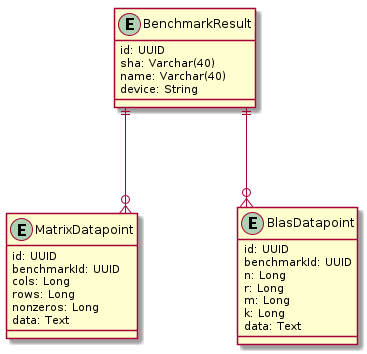
\includegraphics[scale=0.5]{er.png}
	\caption{Entity Relation diagram}
  \label{fig:er}
\end{figure}

The previous database scheme consisted of many tables for each component of a benchmark result. This made the database accesses slow and lead to a very big memory footprint. The new database scheme uses only three tables and is much faster and compacter as a result of that. This was accomplished by storing the data for solvers, formats, operations etc. in JSON format. This only has the downside of adding complexity to the database handler when updating results with new datapoints.


\section{API}

\textbf{/post}
\begin{tabular}{ l l l l }
Name & Type & In & Description \\ 
\hline
sha & String & query & Sha for benchmark result \\
device & String & query & Name for benchmark result \\
blas & Boolean & query & Has to be true when uploading blas benchmark results \\
json & JSON & body & Contains the benchmark data \\
\hline
\end{tabular}




\appendix



\end{document}
